\chapterimage{distribution}
\chapter{Information}\label{sec:info}

The main goal of this chapter is to formalize the concept of \concept{information}
(distinguishing it from plain \concept{data}), and link it to the notion of \concept{compressibility}.

\section{Elements of transmission}\label{sec:info:elements}

\begin{center}
    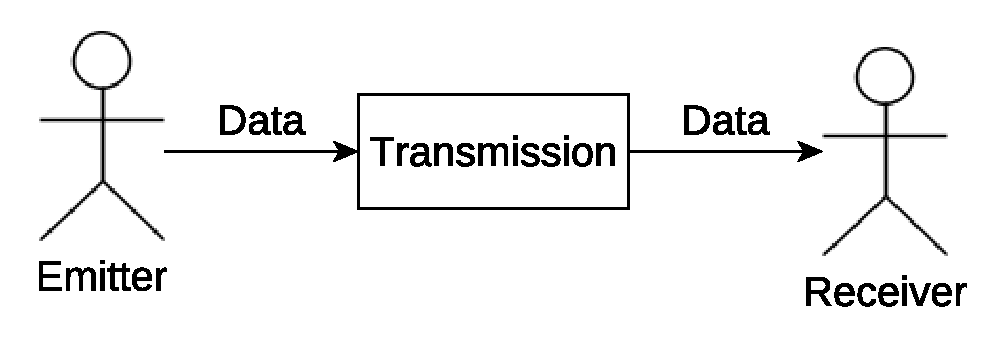
\includegraphics[width=0.5\linewidth]{transmission_basic}
\end{center}

The most simple \concept{transmission} scheme involves an \concept{emitter}, a \concept{receiver}, and the \concept{data} that is
is produced by a \concept{source} and transmitted through a \concept{channel}~\cite{shannon_communication,stone_information}.
Three key aspects of this transmission are its \concept{efficiency}, its \concept{exactness} and its \concept{privacy/authenticity}.
These are typically achieved thanks to the tools provided by, respectively,
\concept{data compression}, \conceptRef{error correcting code}{error correcting codes} and \concept{cryptography}/\concept{computer security}.
This course deals mainly with the first class of tools and their links to the third class.

The \concept{source} \source
is the element that produces a sequence of symbols $s_1,\,s_2,\,\ldots,s_N$
from a finite \concept{alphabet}
$\alphabet = \{\sigma_1,\,\sigma_2,\,\ldots,\sigma_{|\alphabet|}\}$, \ie, $s_i \in \alphabet\ \forall i$.
To characterize the source, we need to know the \concept{probability distribution} of all possible symbols,
\eg, $\Pri\ \forall i$.
Often, symbol \concept{independence} and a constant or \concept{stationary}~\cite[\S 4.1]{sayood_introduction}
distribution during symbol production is assumed for simplicity, although it is not always the case
\cite[\S 2.2]{sayood_introduction}.

Symbols can be expressed using a fixed-length, uncompressed representation, as described in Chapter~\ref{sec:data}.
While simple, this approach is generally not as \conceptRef{efficiency}{efficient} as it could.
\conceptRef{data compression}{Data compression} is the process of expressing a sequence of symbols
in a compact representation more suitable for transmission.
%
There are several strong motivations to use data compression~\cite[\S 1]{sayood_introduction}.
These include limited \concept{bandwidth}, transmission time, storage capacity and overall operational cost.
In each scenario, we need to decide whether to use \concept{lossless compression}~\cite[\S 1.1.1]{sayood_introduction}
or \concept{lossy compression}~\cite[\S 1.1.2]{sayood_introduction}, weighing the pros and cons of each one.


\section{Surprise and entropy}~\label{sec:info:surprise}

When a symbol $\sigma_i$ with probability $\Pri$ is produced by a source, the amount
of \concept{information} (\concept{surprisal}, \aka\ \concept{self-information}),
conveyed by that symbol is
$I(\sigma_i) = \log_2(1/\Pri) = -\log_2(\Pri)$
\conceptRef{bit}{bits}. The more surprising that symbol is (\ie, the lower its probability),
the more informative the appearance of that symbol is.

The \concept{logarithm} in this expression is intuitively motivated by the fact that $B$ bits can be used
to distinguish between $2^B$ equiprobable (\ie, $\Pri = 1/2^B$ symbols), and
the self-information of any of those symbols would be
$I(\sigma_i) = B$ bits~\cite[\S 2.2]{sayood_introduction},\cite[\S VI]{shannon_communication}.
The use of the logarithm also guarantees that the occurrence of two \conceptRef{independence}{independent} symbols
$\sigma_i$ and $\sigma_i$ conveys an amount of information equal to the sum of their
self-informations, \ie,
$I(\sigma_i, \sigma_j) = -\log_2(P(\sigma_i,\sigma_j))
= -\log_2(\Pri P(\sigma_j)) = -\log_2(\Pri) -\log_2(P(\sigma_j)) = I(\sigma_i) + I(\sigma_j).$

The information produced by a \concept{stationary} source is given by the weighted average of
its symbols' self-information~\cite{shannon_communication}, \ie, its \concept{first-order entropy}:
$\entropy(\source) = \sum_i \Pri I(\sigma_i) = - \sum_i \Pri \log_2(\Pri)$.

The \concept{minimum entropy} possible is $0$, which corresponds to the case of a single, deterministic outcome
and no information conveyed.
%
The \concept{maximum entropy} given \alphabet is obtained for the \concept{uniform distribution}
case.
%
Based on this, the upper bound is $\log_2(|\alphabet|)$
bits~\cite[Theorem 2.6.4]{cover_elements},\cite[\S 2.1.2]{taubman2002jpeg2000}.
%
One way to obtain this result is using Lagrangian optimization
\begin{eqnarray*}
J &=& - \sum_{i=1}^{|\alphabet|} \Pri \log_2(\Pri) + \lambda (\sum_{i=1}^{|\alphabet|} \Pri - 1), \\
0 = \frac{\partial J}{\partial \Pri} &=& -(\log_2(\Pri) + 1) + \lambda
\Rightarrow  \Pri = e^{\lambda - 1}, \\
1 = \sum_{i=1}^{|\alphabet|} \Pri &=& |\alphabet| e^{\lambda-1} = |\alphabet| \Pri
\Rightarrow  \Pri = 1/|\alphabet|.
\end{eqnarray*}

%
The maximum entropy case is particularly important when producing \concept{cryptographical keys}
to prevent an attacker from making educated guesses about the chosen key~\cite[Theorem 2.4]{stinson_crypto}.

Real sources don't typically produce symbols \conceptRef{independence}{independently}. Instead,
the probability of the next symbol depends on what symbols have been already
produced~\cite[\S 3]{shannon_communication} (think text or natural images). In this case,
a higher-order entropy definition that considers a \concept{context} of previously observed symbols
is needed to assess the amount of information conveyed. For instance, one can use a context comprising
the previously emitted symbol and calculate $\Pri = \sum_j P(\sigma_j) P(\sigma_i | \sigma_j)$.

\section*{Further reading and practice}
\begin{itemize}
\item \cite{sayood_introduction}: All things data compression, very useful to the course.
It presents things in rigorous but not too mathy way. Freely available (online and offline) for all enrolled students.
Chapters 2.1 and 2.2 are of special interest for this Unit.

\item \cite[\S 3]{mcanlis_understanding}: Section~3 provides a mathematically casual description of
entropy, with minimal math ``interference''. Highly recommended as well.

\item \cite{cover_elements}: A very complete manual on Information Theory, which deals with many of the concepts of the course
from a mathematically rigorous point of view.
It is also freely available online. The following chapters are of special interest for this Unit:
\begin{itemize}
    \item Chapter 2.1: notion of entropy. Read the rest of Chapter 2 for properties and related definitions.
    \item Chapter 3.1: the Asymptotic Equipartition Property Theorem (Theorem 3.1.1), which justifies how we calculate entropy in practice
    \item Chapter 4.2: definition and examples of the entropy rate of a sequence of $n$ variables.
    Read the introduction to Chapter 4 and Chapter 4.1 for more information on sequences of $n$ variables (Markov chains).
\end{itemize}

\item \cite{shannon_communication}: seminal paper by Claude Shannon first describing a theory of communication.
It introduces the main elements of transmission (source, transmitter, channel, uncertainty, entropy, etc.
It is a bit dry, math-oriented and describes many concepts beyond this course, but it is extremely relevant historically.

\item \cite{stone_information}: Relatively gentle description of the contents of Claude Shannon's paper
(\cite{shannon_communication}, see above). Chapters 1 to 4 deal with concepts most relevant to this course.
\end{itemize}


\begin{exercise}
Describe the sources and alphabets that best model the transmission of:
\begin{enumerate}
\item an $8$-bit grayscale image, uncompressed
\item an $8$-bit RGB image, compressed
\item a $12$-bit multispectral image, stored using $2$ bytes per sample
\item a $12$-bit multispectral image, stored using $4$ bytes per sample
\end{enumerate}
\end{exercise}

\begin{exercise}
Model the source that produced the \url{mandrill-u8be-3x512x512.raw} image.
Assume symbol independence.
\end{exercise}

\begin{exercise}
Discuss the preferability of lossless vs. lossy compression in the following \mbox{scenarios}:
\begin{enumerate}
\item Natural images
\item Digital pathology images
\item Remote sensing data
\item Text (\eg, a book)
\item Program code
\item Audio
\end{enumerate}
\end{exercise}

\begin{exercise}
How much information is conveyed by the following experiments:
\begin{enumerate}
\item Flipping $1$ fair coin.
\item Flipping $1$ fair coin, then another.
\item Flipping $2$ fair coins simultaneously.
\item Flipping $1$ fair coin and $1$ fair die.
\item Checking the status of an alarm that is broken (and can never go off).
\item Checking the status of an alarm that is broken (and is constantly going off).
\end{enumerate}
\end{exercise}

\begin{exercise}
How many bits do we need on average to express an outcome of a
binary source ($|\alphabet|=2$) that produces one symbol three times as often as the other?
If the number is not an integer, explain why.
\end{exercise}

\begin{exercise}
Model the source that produced the \url{mandrill-u8be-3x512x512.raw} image
assuming that the probability of each pixel depends on the immediately previous
emitted pixel (and no other pixel).
\end{exercise}
